% ------------------------------------------
\documentclass[automark,a4paper,11pt,headsepline]{scrartcl}
%\usepackage{ngerman}
\topmargin 0 cm
\headheight 0 cm
\headsep 0.9 cm
\oddsidemargin 0 cm
\evensidemargin 0 cm 
\textwidth  16.0 cm 
\textheight 24.6 cm

%\usepackage{fancyhdr} % fancy header
%\pagestyle{fancy}
%%\renewcommand{\chaptermark}[1]{\markboth{#1}{}}
%%\renewcommand{\sectionmark}[1]{\markright{\thesection\ #1}}
%\renewcommand{\sectionmark}[1]{\markright{#1}}
%\fancyhf{}
%\fancyhead[LE,RO]{\bfseries\thepage}
%\fancyhead[LO]{\bfseries\rightmark}
%\fancyhead[RE]{\bfseries\leftmark}
%\renewcommand{\headrulewidth}{0.5pt}
%\renewcommand{\footrulewidth}{0pt} 
%\addtolength{\headheight}{0.5pt}
%\fancypagestyle{plain}{ 
%	\fancyhead{}
%	\renewcommand{\headrulewidth}{0pt} 
%}

\usepackage{graphicx} 
\usepackage{color}
\usepackage[all]{xy}  
\usepackage{hhline}
\usepackage{url}  
\usepackage{alltt}
\usepackage{amsmath} 
\usepackage{amssymb}  
%\numberwithin{equation}{chapter}
\usepackage{hyperref}
\hypersetup{
    bookmarks=true,         % show bookmarks bar?
    unicode=false,          % non-Latin characters in Acrobat’s bookmarks
    pdftoolbar=true,        % show Acrobat’s toolbar?
    pdfmenubar=true,        % show Acrobat’s menu?
    pdffitwindow=true,      % page fit to window when opened
    pdftitle={My title},    % title
    pdfauthor={Author},     % author
    pdfsubject={Subject},   % subject of the document
    pdfnewwindow=true,      % links in new window
    pdfkeywords={keywords}, % list of keywords
    colorlinks=true,        % false: boxed links; true: colored links
    linkcolor=black,        % color of internal links
    citecolor=blue,         % color of links to bibliography
    filecolor=blue,         % color of file links
    urlcolor=blue           % color of external links
}


\renewcommand{\vec}[1]{\boldsymbol{#1}}
\newcommand{\bs}[1]{\mathbf #1} 
\newcommand{\der}[1]{\mathtt{d}#1}
\newcommand{\pri}[1]{#1^{\prime}}
\newcommand{\curl}[1]{\mathbf \nabla \wedge \vec{#1}}

\newsavebox{\fmbox}
\definecolor{lightgray}{gray}{0.95}
\newenvironment{fmpage}
   {\vspace{-0.40cm}\begin{lrbox}{\fmbox}\begin{minipage}[t]{15.5cm}\vspace{0.1cm}}
   {\vspace{-0.4cm}\end{minipage}\end{lrbox}\begin{center}\fcolorbox{black}{lightgray}{\usebox{\fmbox}}\end{center}}

\author{Christof Kraus}
\title{Auto Phasing in OPAL-T}
\begin{document}
\maketitle

\section{Standing Wave Cavity}
In OPAL-T the elements are implemented as external fields that are read in from a file. The fields are described by a 1D, 2D or 3D sampling (equidistant or non-equidistant). To get the actual field at any position a linear interpolation multiplied by $\cos(\omega t + \varphi)$, where $\omega$ is the frequency and $\varphi$ is the lag. The energy gain of a particle then is
\begin{equation}
\Delta E(\varphi,r) = q\,V_{0}\,\int_{z_\text{begin}}^{z_\text{end}} \cos(\omega t(z,\varphi) + \varphi) E_z(z, r) dz.
\end{equation}
To maximize the energy gain we have to take the derivative with respect to the lag, $\varphi$ and set the result to zero:
\begin{multline}
\frac{d\, \Delta E(\varphi,r)}{d\,\varphi} = -\int_{z_\text{begin}}^{z_\text{end}} (1 + \omega \frac{\partial\,t(z,\varphi)}{\partial\,\varphi}) \sin(\omega t(z,\varphi) + \varphi) E_z(z,r)\\
= -\cos(\varphi) \int_{z_\text{begin}}^{z_\text{end}} (1 + \omega \frac{\partial\,t(z,\varphi)}{\partial\,\varphi}) \sin(\omega t(z,\varphi)) E_z(z,r) dz \\
-\sin(\varphi) \int_{z_\text{begin}}^{z_\text{end}} (1 + \omega \frac{\partial\,t(z,\varphi)}{\partial\,\varphi}) \cos(\omega t(z,\varphi)) E_z(z,r) dz \stackrel{!}{=} 0.
\end{multline}
Thus to get the maximum energy the lag has to fullfill 
\begin{equation} \label{eqn:rulelag}
  \tan(\varphi) = -\frac{\Gamma_1}{\Gamma_2},
\end{equation}
where 
\begin{equation}
  \label{eqn:Gamma1}
  \Gamma_1 = \sum_{i=1}^{N-1} (1 + \omega \frac{\partial\,t}{\partial\,\varphi}) \int_{z_{i-1}}^{z_{i}} \sin\left(\omega (t_{i-1} + \Delta t_{i}\frac{z-z_{i-1}}{\Delta z_{i}})\right)\left(E_{z,i-1} + \Delta E_{z,i} \frac{z-z_{i-1}}{\Delta z_{i}}\right) dz
\end{equation}
and
\begin{equation}
  \label{eqn:Gamma2}
  \Gamma_2 = \sum_{i=1}^{N-1} (1 + \omega \frac{\partial\,t}{\partial\,\varphi}) \int_{z_{i-1}}^{z_{i}} \cos\left(\omega (t_{i-1} + \Delta t_{i}\frac{z-z_{i-1}}{\Delta z_{i}})\right)\left(E_{z,i-1} + \Delta E_{z,i} \frac{z-z_{i-1}}{\Delta z_{i}}\right) dz.
\end{equation}
Between two sampling points we assume a linear correlation between the electric field and position respectively between time and position. The products in the  integrals between two sampling points can be expanded and solved analytically. We then find
\begin{equation*}
\Gamma_1 = \sum_{i=1}^{N-1} (1 + \omega \frac{\partial\,t}{\partial\,\varphi}) \Delta z_{i}(E_{z,i-1} (\Gamma_{11,i} - \Gamma_{12,i}) + E_{z,i}\, \Gamma_{12,i})
\end{equation*}
and
\begin{equation*}
\Gamma_1 = \sum_{i=1}^{N-1} (1 + \omega \frac{\partial\,t}{\partial\,\varphi}) \Delta z_{i}(E_{z,i-1} (\Gamma_{21,i} - \Gamma_{22,i}) + E_{z,i}\, \Gamma_{22,i})
\end{equation*}
where
\begin{align*}
  \Gamma_{11,i} &= \int_0^1 \sin(\omega(t_{i-1} + \tau \Delta t_{i})) d\tau = - \frac{\cos(\omega t_{i}) - \cos(\omega t_{i-1})}{\omega \Delta t_{i}}\\
  \Gamma_{12,i} &= \int_0^1 \sin(\omega(t_{i-1} + \tau \Delta t_{i})) \tau d\tau = \frac{-\omega \Delta t_{i} \cos(\omega t_{i}) + \sin(\omega t_{i}) - \sin(\omega t_{i-1})}{\omega^2 (\Delta t_{i})^2}\\
  \Gamma_{21,i} &= \int_0^1 \cos(\omega(t_{i-1} + \tau \Delta t_{i})) d\tau = \frac{\sin(\omega t_{i}) - \sin(\omega t_{i-1})}{\omega \Delta t_{i}}\\
  \Gamma_{22,i} &= \int_0^1 \cos(\omega(t_{i-1} + \tau \Delta t_{i})) \tau d\tau = \frac{\omega \Delta t_{i} \sin(\omega t_{i}) + \cos(\omega t_{i}) - \cos(\omega t_{i-1})}{\omega^2 (\Delta t_{i})^2}
\end{align*}

It remains to find the progress of time with respect to the position. In OPAL this is done iteratively starting with 
\begin{verbatim}
K[i] = K[i-1] + (z[i] - z[0]) * q * V;
b[i] = sqrt(1. - 1. / ((K[i] - K[i-1]) / (2.*m*c^2) + 1)^2);
t[i] = t[0] + (z[i] - z[0]) / (c * b[i])
\end{verbatim}
By doing so we assume that the kinetic energy, K, increases linearly and proportional to the maximal voltage. With this model for the progress of time we can calculate $\varphi$ according to Equation~\ref{eqn:rulelag}. Next a better model for the kinetic Energy can be calculated using 
\begin{alltt}
K[i] = K[i-1] + q \(\Delta\)z[i](cos(\(\varphi\))(Ez[i-1](\(\Gamma\sb{21}\)[i] - \(\Gamma\sb{22}\)[i]) + Ez[i]\(\Gamma\sb{22}\)[i]) 
                      \(\,\,\)- sin(\(\varphi\))(Ez[i-1](\(\Gamma\sb{11}\)[i] - \(\Gamma\sb{12}\)[i]) + Ez[i]\(\Gamma\sb{12}\)[i])).
\end{alltt}
With the updated kinetic energy the time model and finally a new $\varphi$, that comes closer to the actual maximal kinetic energy, can be obtained. One can iterate a few times through this cycle until the value of $\varphi$ has converged.

\section{Traveling Wave Structure}
\begin{figure} 
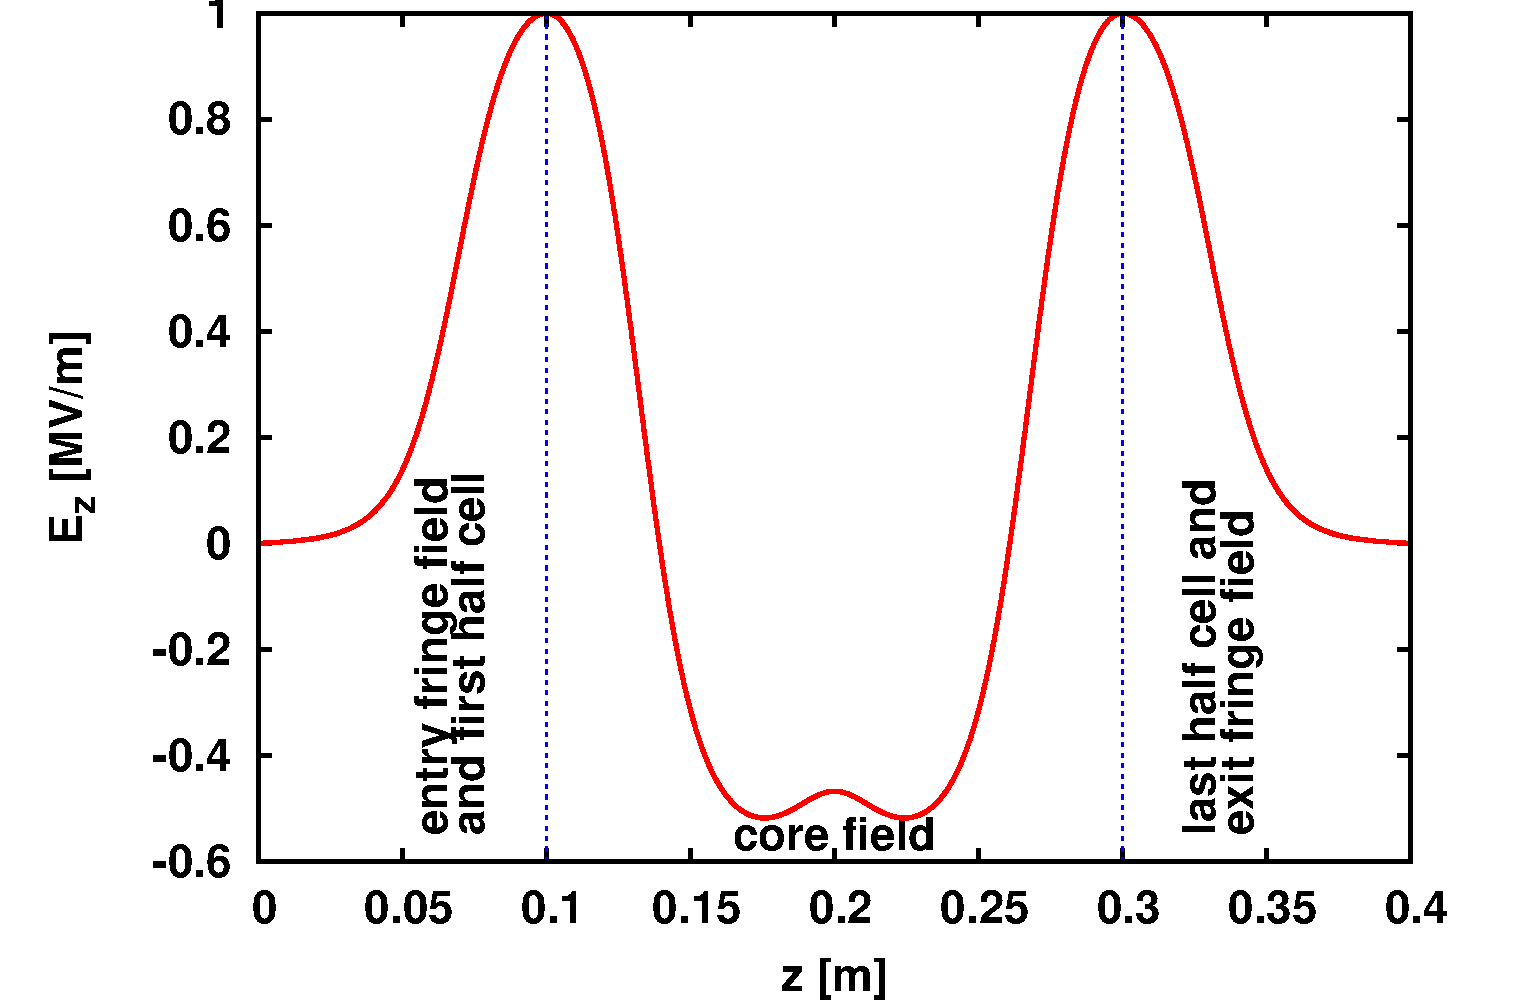
\includegraphics[angle=0,width=0.9\linewidth]{field_crop}
\caption{Field map 'FINLB02-RAC.T7' of type 1DDynamic}
\label{tws}
\end{figure}
Auto phasing in a traveling wave structure is just slightly more complicated. The field of this element is composed of a standing wave entry and exit fringe field and two standing waves in between, see Figure~\ref{tws}.
\begin{multline}
\Delta E(\varphi,r) = q\, V_{0}\,\int_{z_\text{begin}}^{z_\text{beginCore}} \cos(\omega t(z,\varphi) + \varphi) E_z(z, r) dz \\
+ q\, V_\text{core}\,\int_{z_\text{beginCore}}^{z_\text{endCore}} \cos(\omega t(z,\varphi) + \varphi_\text{c1} + \varphi) E_z(z, r) dz \\
+ q\, V_\text{core}\,\int_{z_\text{beginCore}}^{z_\text{endCore}} \cos(\omega t(z,\varphi) + \varphi_\text{c2} + \varphi) E_z(z + s, r) dz \\
+ q\, V_{0}\,\int_{z_\text{endCore}}^{z_\text{end}} \cos(\omega t(z,\varphi) + \varphi_\text{ef} + \varphi) E_z(z, r) dz,
\end{multline}
where $s$ is the cell length. Instead of one sum as in Equation~(\ref{eqn:Gamma1}) and Equation~(\ref{eqn:Gamma2}) there are four sums with different numbers of summands.
\subsection*{Example}
\begin{fmpage}
\begin{verbatim}
FINLB02_RAC: TravelingWave, L=2.80, VOLT=14.750*30/31, NUMCELLS=40,
             FMAPFN="FINLB02-RAC.T7", ELEMEDGE=2.67066, MODE=1/3,
             FREQ=1498.956, LAG=FINLB02_RAC_lag;
\end{verbatim}
\end{fmpage}
For this example we find
\begin{align*}
  V_\text{core} &= \frac{V_{0}}{\sin(2.0/3.0 \pi)} = \frac{2 V_{0}}{\sqrt{3.0}}\\
  \varphi_\text{c1} &= \frac{\pi}{6}\\
  \varphi_\text{c2} &= \frac{\pi}{2}\\
  \varphi_\text{ef} &= - 2\pi \cdot(\text{NUMCELLS} - 1) \cdot \text{MODE} = 26\pi
\end{align*}
\subsection{Alternative Approache for Traveling Wave Structures}
If $\beta$ doesn't change much along the traveling wave structure (ultra relativistic case) then $t(z,\varphi)$ can be approximated by $t(z,\varphi)=\frac{\omega}{\beta c}z + t_{0}$. For the example from above the energy gain is approximately
\begin{multline*}
\Delta E(\varphi,r) = q\;V_0 \int_{0}^{1.5\cdot s} \cos\left(\omega \left(\frac{z}{\beta c} + t_{0}\right) + \varphi\right) E_z(z,r)\, dz\\
+ \frac{2 q\;V_{0}}{\sqrt{3}} \int_{1.5\cdot s}^{40.5\cdot s}\cos\left(\omega \left(\frac{z}{\beta c} + t_{0}\right) + \frac{\pi}{6} + \varphi \right) E_z(z\;\;\quad,r) dz\\
+ \frac{2 q\;V_{0}}{\sqrt{3}} \int_{1.5\cdot s}^{40.5\cdot s}\cos\left(\omega \left(\frac{z}{\beta c} + t_{0}\right) + \frac{\pi}{2} + \varphi \right) E_z(z+s,r) dz \\
  + q\;V_{0} \int_{40.5\cdot s}^{42\cdot s} \cos\left(\omega \left(\frac{z}{\beta c} + t_{0}\right) + \varphi\right) E_z(z,r)\, dz.
\end{multline*}
Here $\beta c = 2.9886774\cdot10^8\;\text{m s}^{-2}$, $\omega = 2\pi\cdot 1.4989534\cdot10^9$~Hz and, the cell length, $s = 0.06\bar{6}$~m. To maximize this energy we have to take the derivative with respect to $\varphi$ and set the result to $0$. We split the field up into the core field, $E_z^{(1)}$ and the fringe fields (entry fringe field plus first half cell concatenated with the exit fringe field plus last half cell), $E_z^{(2)}$. The core fringe field is periodic with a period of $3\,s$. We thus find
\begin{multline*}
0 \stackrel{!}{=} \int_{0}^{1.5\cdot s} \sin\left(\omega \left(\frac{z}{\beta c} + t_{0}\right) + \varphi\right) E_z^{(2)}(z,r)\, dz \\
                + \frac{2}{\sqrt{3}} \int_{0}^{39\cdot s}\sin\left(\omega \left(\frac{z + 1.5\,s}{\beta c} + t_{0}\right) + \frac{\pi}{6} + \varphi \right) E_z^{(1)}(z \text{ mod}(3\,s)\;\;\qquad,r)\,dz \\
                + \frac{2}{\sqrt{3}} \int_{0}^{39\cdot s}\sin\left(\omega \left(\frac{z + 1.5\,s}{\beta c} + t_{0}\right) + \frac{\pi}{2} + \varphi \right) E_z^{(1)}((z + s) \text{ mod} (3\,s),r)\, dz \\
                + \int_{1.5\cdot s}^{3\cdot s} \sin\left(\omega\left(\frac{z + 39\,s}{\beta c} + t_{0}\right) + \varphi\right) E_z^{(2)}(z,r)\, dz
\end{multline*}
This equation is much simplified if we take into account that $\omega / \beta c \approx 10\pi$. We then get
\begin{multline*}
0 \stackrel{!}{=} \int_{0}^{3\cdot s} \sin\left(\omega \left(\frac{z}{\beta c} + t_{0}\right) + \varphi\right) E_z^{(2)}(z)\, dz \\
                + \frac{26}{\sqrt{3}} \int_{0}^{3\cdot s}\left(\sin\left(\omega \left(\frac{z}{\beta c} + t_{0}\right) + \frac{7\pi}{6} + \varphi \right) 
                                                        + \sin\left(\omega \left(\frac{z}{\beta c} + t_{0}\right) + \frac{5\pi}{6} + \varphi \right)\right) E_z^{(1)}(z)\, dz \\
       = \int_{0}^{3\cdot s}\sin\left(\omega \left(\frac{z}{\beta c} + t_{0}\right) + \varphi\right) \left(E_z^{(2)} - 26\cdot E_z^{(1)}\right)(z)\,dz
\end{multline*}
where we used
\begin{multline*}
\int_{0}^{3\cdot s} \sin\left(\omega \left(\frac{z}{\beta c} + t_{0}\right) + \frac{3\pi}{2} + \varphi\right) E_z^{(1)}((z + s) \text{ mod}(3\,s),r) dz \\
\stackrel{z' = z + s}{\longrightarrow} \int_{s}^{4\cdot s} \sin\left(\omega \left(\frac{z'-s}{\beta c} + t_{0} \right) + \frac{3\pi}{2} + \varphi\right)E_z^{(1)}(z' \text{ mod}(3\,s),r)dz' \\ 
= \int_{0}^{3\cdot s} \sin\left(\omega \left(\frac{z}{\beta c} + t_{0}\right) + \frac{5\pi}{6} + \varphi\right) E_z^{(1)}(z,r)\,dz.
\end{multline*}
In the last equal sign we used the fact that both functions, $\sin(\frac{\omega}{\beta c}z)$ and $E_z^{(1)}$ have a periodicity of $3\cdot s$ to shift the boundaries of the integral.

Using the convolution theorem we find
\begin{equation*}
0 \stackrel{!}{=} \int_{0}^{3\cdot s} g(\xi - z) (G - 26 \cdot H)(z) \, dz = 
\mathcal{F}^{-1}\left(\mathcal{F}(g)\cdot(\mathcal{F}(G) - 26 \cdot \mathcal{F}(H))\right)
\end{equation*}
where
\begin{align*}
  g(z) & = 
  \begin{cases}
    -\sin\left(\omega \left(\frac{z}{\beta c} + t_{0}\right)\right)\qquad & 0 \le z \le 3\cdot s\\
    0                                     & \text{otherwise}
  \end{cases}\\
  G(z) & =
  \begin{cases}
    E_z^{(2)}(z) \qquad & 0 \le z \le 3\cdot s\\
    0                   & \text{otherwise}
  \end{cases}\\
  H(z) & =
  \begin{cases}
    E_z^{(1)}(z) \qquad & 0 \le z \le 3\cdot s\\
    0                   & \text{otherwise}
  \end{cases}
  \intertext{and}
  -\frac{\omega}{\beta c} \xi &= \varphi.
\end{align*}
Here we also used some trigonometric identies:
\begin{multline*}
  \sin\left(\omega \left(\frac{z}{\beta c} + t_{0}\right) + \pi + \frac{\pi}{6} + \varphi \right) + 
  \sin\left(\omega \left(\frac{z}{\beta c} + t_{0}\right) + \pi - \frac{\pi}{6} + \varphi \right) \\
  = -\left(\sin\left(\omega \left(\frac{z}{\beta c} + t_{0}\right) + \frac{\pi}{6} + \varphi\right) + 
    \sin\left(\omega \left(\frac{z}{\beta c} + t_{0}\right) - \frac{\pi}{6} + \varphi\right)\right) \\
  = -2\cdot \cos\left(\frac{\pi}{6}\right) \sin\left(\omega \left(\frac{z}{\beta c} + t_{0}\right) + \varphi\right) \\
  = -\sqrt{3} \sin\left(\omega \left(\frac{z}{\beta c} + t_{0}\right) + \varphi\right)
\end{multline*}
\end{document} 
  

 

% LocalWords:  undulator undulatory CSR emittance XFEL ansatz paraxial gauge IP
% LocalWords:  discretized lossy FETD FDTD CFL Yee subgridding indices Nyquist
% LocalWords:  subgrids PEC IPPL parallelized FEL symplectic CSCS LANL SciDAC
% LocalWords:  Parallelization benchmarked Adelmann Scherrer Institut Betatron
% LocalWords:  LBNL Saldin Schneidmiller Yurkov Nucl Meth Dohlus Kabel Limberg
% LocalWords:  Agoh Yokoya Accel Stupakov Kotelnikov IEEE Technol Lett Shlager
% LocalWords:  Maloney Taflove Hagness Nowood Artech Hiptmair ETH Donderici Nr
% LocalWords:  Teixeira Wittberger Qiang Ryne Limborg Deprey Diss joachim Appl
% LocalWords:  Mech Engrg
